\documentclass{article}\usepackage[]{graphicx}\usepackage[]{color}
%% maxwidth is the original width if it is less than linewidth
%% otherwise use linewidth (to make sure the graphics do not exceed the margin)
\makeatletter
\def\maxwidth{ %
  \ifdim\Gin@nat@width>\linewidth
    \linewidth
  \else
    \Gin@nat@width
  \fi
}
\makeatother

\definecolor{fgcolor}{rgb}{0.345, 0.345, 0.345}
\newcommand{\hlnum}[1]{\textcolor[rgb]{0.686,0.059,0.569}{#1}}%
\newcommand{\hlstr}[1]{\textcolor[rgb]{0.192,0.494,0.8}{#1}}%
\newcommand{\hlcom}[1]{\textcolor[rgb]{0.678,0.584,0.686}{\textit{#1}}}%
\newcommand{\hlopt}[1]{\textcolor[rgb]{0,0,0}{#1}}%
\newcommand{\hlstd}[1]{\textcolor[rgb]{0.345,0.345,0.345}{#1}}%
\newcommand{\hlkwa}[1]{\textcolor[rgb]{0.161,0.373,0.58}{\textbf{#1}}}%
\newcommand{\hlkwb}[1]{\textcolor[rgb]{0.69,0.353,0.396}{#1}}%
\newcommand{\hlkwc}[1]{\textcolor[rgb]{0.333,0.667,0.333}{#1}}%
\newcommand{\hlkwd}[1]{\textcolor[rgb]{0.737,0.353,0.396}{\textbf{#1}}}%

\usepackage{framed}
\makeatletter
\newenvironment{kframe}{%
 \def\at@end@of@kframe{}%
 \ifinner\ifhmode%
  \def\at@end@of@kframe{\end{minipage}}%
  \begin{minipage}{\columnwidth}%
 \fi\fi%
 \def\FrameCommand##1{\hskip\@totalleftmargin \hskip-\fboxsep
 \colorbox{shadecolor}{##1}\hskip-\fboxsep
     % There is no \\@totalrightmargin, so:
     \hskip-\linewidth \hskip-\@totalleftmargin \hskip\columnwidth}%
 \MakeFramed {\advance\hsize-\width
   \@totalleftmargin\z@ \linewidth\hsize
   \@setminipage}}%
 {\par\unskip\endMakeFramed%
 \at@end@of@kframe}
\makeatother

\definecolor{shadecolor}{rgb}{.97, .97, .97}
\definecolor{messagecolor}{rgb}{0, 0, 0}
\definecolor{warningcolor}{rgb}{1, 0, 1}
\definecolor{errorcolor}{rgb}{1, 0, 0}
\newenvironment{knitrout}{}{} % an empty environment to be redefined in TeX

\usepackage{alltt}

\usepackage{fancyhdr} % Required for custom headers
\usepackage{lastpage} % Required to determine the last page for the footer
\usepackage{extramarks} % Required for headers and footers
\usepackage{graphicx} % Required to insert images
\usepackage{hyperref}
\usepackage{amsmath} %for binomial pdf
\usepackage{parskip} % so that there's space bw paragraphs
\usepackage{float}
\usepackage{amsfonts}

% Margins
\topmargin=-0.45in
\evensidemargin=0in
\oddsidemargin=0in
\textwidth=6.5in
\textheight=9.0in
\headsep=0.25in 

\linespread{1.1} % Line spacing

% Set up the header and footer
\pagestyle{fancy}
\lhead{STAT 532: Bayes} % Top left header
\chead{HW 4} % Top center header
\rhead{Andrea Mack} % Top right header
\lfoot{10/10/2016} % Bottom left footer
\cfoot{} % Bottom center footer
\rfoot{Page\ \thepage\ of\ \pageref{LastPage}} % Bottom right footer
\renewcommand\headrulewidth{0.4pt} % Size of the header rule
\renewcommand\footrulewidth{0.4pt} % Size of the footer rule

\setlength\parindent{0pt} % Removes all indentation from paragraphs
\setlength\parskip{0.5cm}
\restylefloat{table}

%----------------------------------------------------------------------------------------
%	DOCUMENT STRUCTURE COMMANDS
%	Skip this unless you know what you're doing
%----------------------------------------------------------------------------------------

% Header and footer for when a page split occurs within a problem environment
\newcommand{\enterProblemHeader}[1]{
\nobreak\extramarks{#1}{#1 continued on next page\ldots}\nobreak
\nobreak\extramarks{#1 (continued)}{#1 continued on next page\ldots}\nobreak
}

% Header and footer for when a page split occurs between problem environments
\newcommand{\exitProblemHeader}[1]{
\nobreak\extramarks{#1 (continued)}{#1 continued on next page\ldots}\nobreak
\nobreak\extramarks{#1}{}\nobreak
}


%----------------------------------------------------------------------------------------%
\IfFileExists{upquote.sty}{\usepackage{upquote}}{}
\begin{document}


\begin{enumerate}
\item%1 
{\it (5 points) How do Monte Carlo and Markov Chain Monte Carlo (MCMC) procedures differ?}

MC procedures involve sampling from the marginal posterior distribution p($\sigma^2 | y_{\sim}$) and using that value to sample from the full conditional p($\theta | \sigma^2, y_{\sim}$). All $\sigma^2$ are independently drawn, making each set $\phi$ = {$\theta_{i}$, $\sigma^2_{i}$} independent.

MCMC differs in that apart from the starting value of $\sigma^2$, $\theta_{i}$ and $\sigma^2_{i}$ are iteratively sampled from their respective full conditional posterior distributions. In MCMC, each iteration is dependent on the previous one, and only the previous one. Conditional on the previous set of outcomes, the current set of outcomes is independent of all other previous sets of outcomes - ``a signifying property of a Markov Chain". 

MC procedures have perfect mixing, because each sample is independent of the previous one. In MCMC procedures, the larger the number of simulations, the more likely that mixing has occured.


{\it Side note: It seems that estimates from iterations more than ``one lag" apart would be correlated. -- From class: the algorithm only uses the input from the previous iteration, and doesn't account for the fact that the previous iteration depended on say the (n-2)th iteration.}


\item {\it (5 points) How are the full conditional distributions used in a Gibbs Sampler?}

The full conditional distributions are used iteratively such that the random outcome from one full conditional becomes the input for the full conditional on the other parameter.  

The idea is to approximate the joint distribution p($\theta,\sigma^2 | y_{\sim}$) with p($\theta_{i+1} |\sigma^2_{i},y_{\sim}$)*p($\sigma^2_{i}|\theta_{i},y_{\sim}$) from many pairs of $\theta_{i}$ and $\sigma^2_{i}$'s. 

\item%3 
{\it (5 points) How do the marginal and conditional posterior distributions differ?}

A marginal posterior distribution is a pdf of the parameter of interest conditional on the data, for example, p($\theta | y_{\sim}$). A conditional posterior is a pdf of the parameter of interst conditional on other parameters and conditional on the data, for example, p($\theta|\sigma^2,y_{i}$). The difference is that the marginal posterior is not conditioned on other parameters, while the conditional is conditioned on other parameters. MC uses a marginal posterior distribution on the precison and MCMC uses a conditional posterior distribution on the precision.

\item %4
{\it (5 points) How do you visually assess convergence of an MCMC algorithm?}

To visually assess convergence of an MCMC algorithm, a trace plot of the outcomes should show movement from lower to higher density regions, so that outcomes are not ``stuck" in one region .

With a trace plot, convergence would be met if the distribution of the chains is consistent as the number of iterations increase.

\item %5 
{\it (5 points) Explain the idea of the effective sample size of an MCMC algorithm.}
Let $\phi$ = the variance of the parameter set

$Var_{MCMC}[\phi]$ = $Var_{MC}[\phi]$ + f(autocorrelation)

where f(autocorrelation) is a function of the autocorrelation and usually positive, the variance of MCMC approximations are generally larger than the variance of MC estimates.

If a researcher is interested in a minimum $Var_{MCMC}[\phi]$, we can find S=number of samples such that the $Var_{MC}[\phi]$ = $\frac{\sigma^2}{S}$ = minimum $Var_{MCMC}[\phi]$. The value of S that permits the equality is the effective sample size.

Having a minimum variance of $Var_{MCMC}[\phi]$ is like estimating the $Var_{MC}[\phi]$ from a sample size of the effective sample size.

\item %6
{\it (15 points) Sketch out the steps for a Gibbs sampler algorithm.}

0. Choose an initial $\sigma_{o}^2$ to begin with.

1. Randomly draw a $\theta$ from the full conditional, $\theta|\sigma^2_{i}, y_{\sim}$ ~ N($\mu, \frac{\sigma_{i}^2}{n}$), denoted $\theta_{i}$ and note the first iteration, $\sigma^2_{i} = \sigma^2_{o}$

2.  Randomly draw a $\sigma^2$ from the full conditional, $\sigma^2|\theta_{i}, y_{\sim}$ ~ INVGAM, denoted $\sigma^2_{i}$

3. Iteratively repeat steps (1) and (2), using $\sigma^2_{i}$ in place of $\sigma_{o}$ until approximations achieve convergence and proper mixing

\item %7
{\it Simulating data is a key step in verifying your algorithms are working correctly. This will be
more apparent as we start studying sophisticated hierarchical models.}
\begin{enumerate}
\item%7a
{\it (10 points) Simulate 100 observations from a standard normal distribution and plot a his-
togram of your data.}

\begin{knitrout}
\definecolor{shadecolor}{rgb}{0.969, 0.969, 0.969}\color{fgcolor}
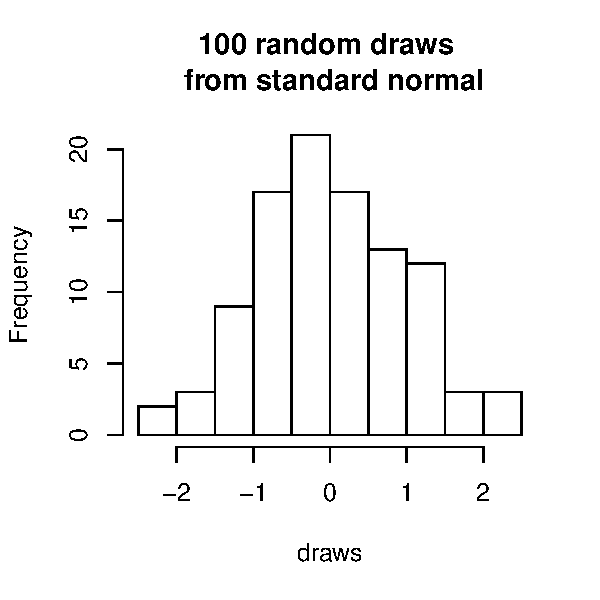
\includegraphics[width=\maxwidth]{figure/prob7a-1} 

\end{knitrout}

\item%7b
{\it (10 points) Select and state prior distributions for $\theta$ the mean of the normal distribution
and $\sigma^2$ the variance (or alternatively you may parameterize your model using the precision
term).}

Below is what you would set up for an MC sampler. In problem (c) I wrote out what I would start with for the Gibbs sampler.

PRIOR DISTRIBUTIONS

$\theta | \sigma^2 \sim$ N($\mu, \frac{\sigma^2}{\kappa_{o}}$)

$\frac{1}{\sigma^2} \sim$ GAM($\frac{\nu_{o}}{2}, \frac{\nu_{o}\sigma_{o}^2}{2}$)

Let $\mu$ = 0
    $\sigma_{o}$ = var(prior samples) = 1, I'm assuming this cannot be taken from the var($y_{\sim}$)       where y was generated in part (a)

    $\kappa_{o}$ = ``hypothetical" sample size = 1, bigger = more informative prior on $\theta$
    
    $\nu_{o}$ = number prior samples = 1, bigger = more informative prior on $\sigma^s$
    
\item %7c
{\it (20 points) Implement a Gibbs sampler to simulate from the joint posterior distribution
p($\theta, \sigma^2 | y_{1}, \cdot, y_{100}$). Create a plot of the joint posterior distribution.}

To set up full conditionals on the parameters of a normal distribution, the distributions are more complicated than in part (b). We generally have to use the Gibbs sampler and the product of the full conditionals to estimate the joint posterior when the variance of the prior on $\theta$ is not directly proportional to $\sigma^2$, making closed form solutions to the posteriors more difficult to find.

$\theta | \sigma^2 \sim$ N($\mu_{n}, \tau_{n}^2$)

$\sigma^2 | \theta \sim$ INVGAM($\frac{\nu_{n}}{2}, \frac{\nu_{n}\sigma^2_{n}}{2}$)

$\mu_{n} = \frac{\frac{\mu_{o}}{\tau_{o}^2} + \frac{n*ybar}{\sigma^2_{n}}}{\frac{1}{\tau_{o}^2} + n*\sigma^2}$

$\tau^2_{n} = (\frac{1}{\tau_{o}^2} + \frac{n}{\sigma^2})^{-1}$

$\nu_{n} = \nu_{o} + n$

$\sigma^2_{n}(\theta) = \frac{1}{\nu_{n}}*[\nu_{o}\sigma_{o}^2 + ns^2_{n}(\theta)]$

$s^2_{n}(\theta) = \frac{\Sigma(y_{i} - \theta)^2}{n}$

$\tau_{o}$ = $\frac{\sigma_{o}}{n}$

Let n = 100, $\nu_{o}$ = 1, $\sigma^2_{o}$ = 1,$\mu_{o}$ = 0, and $\tau^2_{o}$ = 1 which would suggest an uninformative prior, as I don't have prior knowledge or information.

Generate $y_{i}$ from a standard normal distribution.



\begin{knitrout}
\definecolor{shadecolor}{rgb}{0.969, 0.969, 0.969}\color{fgcolor}

{\centering 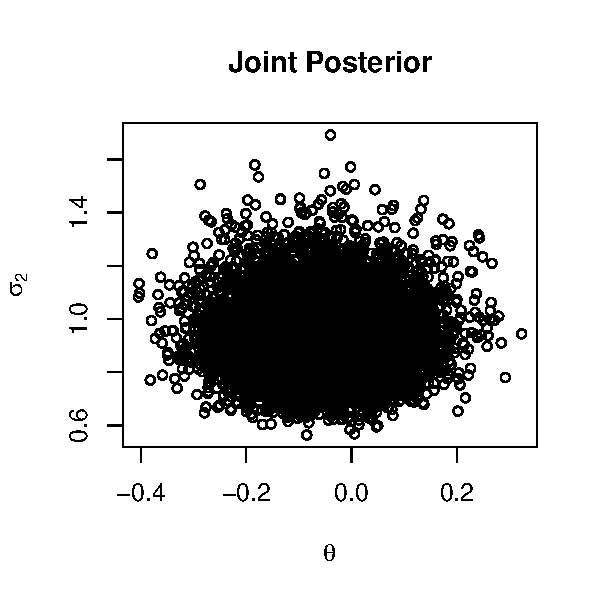
\includegraphics[width=\maxwidth]{figure/prob7cx-1} 

}



\end{knitrout}



\newpage


\item %7d

{\it (10 points) Use your MCMC samples to create a posterior predictive distribution. Compare the data and your posterior predictive distribution using a QQ plot qqnorm(.).
Comment on the figure.}



{\centering 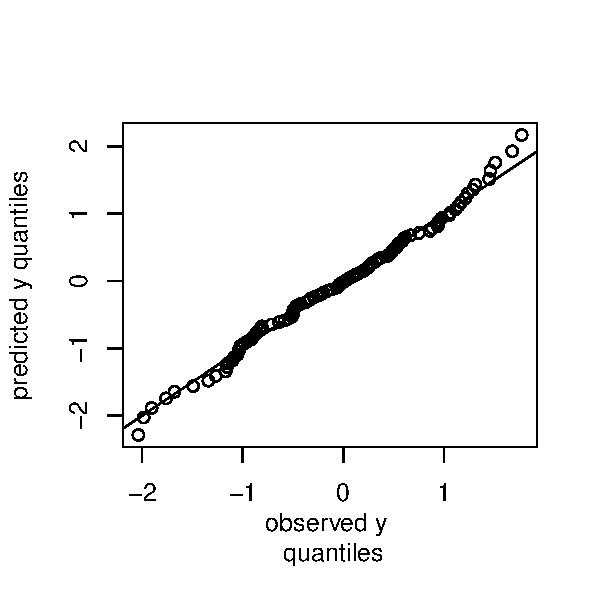
\includegraphics[width=\maxwidth]{figure/prob7d-1} 

}


% latex table generated in R 3.3.1 by xtable 1.8-2 package
% Mon Oct 10 11:37:36 2016
\begin{table}[ht]
\centering
\begin{tabular}{rrr}
  \hline
 & Var(y) & Vary(ystar) \\ 
  \hline
1 & 0.91 & 0.93 \\ 
   \hline
\end{tabular}
\end{table}


The QQplot shows that the quantiles of the posterior predicted values are almost exactly the same as the quantiles from the intially generated data, with slight deviations in the left tail. If I had used a more informative prior, there should be less of a relationship between the quantiles. The table shows there was more variation in the predictions than in the originally generated y's, which is what was expected. The posterior predictive distribution is doing a good job of approximating the distribution of the original y's.
    

\end{enumerate}

\end{enumerate}

\appendix
\section*{R Code}

\begin{enumerate}

\setcounter{enumi}{6}
\item%7
\begin{enumerate}
\item%7a
\begin{knitrout}
\definecolor{shadecolor}{rgb}{0.969, 0.969, 0.969}\color{fgcolor}\begin{kframe}
\begin{alltt}
\hlkwd{set.seed}\hlstd{(}\hlnum{53204}\hlstd{)}
\hlstd{y} \hlkwb{<-} \hlkwd{rnorm}\hlstd{(}\hlnum{100}\hlstd{,}\hlnum{0}\hlstd{,}\hlnum{1}\hlstd{)}

\hlkwd{hist}\hlstd{(y,} \hlkwc{main} \hlstd{=} \hlstr{"100 random draws \textbackslash{}n from standard normal"}\hlstd{,} \hlkwc{xlab} \hlstd{=} \hlstr{"draws"}\hlstd{)}
\end{alltt}
\end{kframe}
\end{knitrout}
\addtocounter{enumii}{1}
\item %7c
\begin{knitrout}
\definecolor{shadecolor}{rgb}{0.969, 0.969, 0.969}\color{fgcolor}\begin{kframe}
\begin{alltt}
\hlcom{# this is my code, and I could not get it to work}
\hlkwd{set.seed}\hlstd{(}\hlnum{53204}\hlstd{)}
\hlstd{n} \hlkwb{<-} \hlnum{100}
\hlstd{y} \hlkwb{<-} \hlkwd{rnorm}\hlstd{(n,}\hlnum{0}\hlstd{,}\hlnum{1}\hlstd{)}

\hlstd{nuo} \hlkwb{<-} \hlnum{1}
\hlstd{nun} \hlkwb{<-} \hlstd{nuo} \hlopt{+} \hlstd{n}
\hlstd{so} \hlkwb{<-} \hlnum{1}
\hlstd{mo} \hlkwb{<-} \hlnum{1}
\hlstd{tau2o} \hlkwb{<-} \hlstd{so}\hlopt{/}\hlstd{n}


\hlstd{precision} \hlkwb{<-} \hlkwd{c}\hlstd{(}\hlkwd{rep}\hlstd{(}\hlnum{0}\hlstd{,n}\hlopt{+}\hlnum{1}\hlstd{))}
\hlstd{t} \hlkwb{<-} \hlkwd{c}\hlstd{(}\hlkwd{rep}\hlstd{(}\hlnum{0}\hlstd{,n))}

\hlstd{tau2n} \hlkwb{<-} \hlkwd{c}\hlstd{(}\hlkwd{rep}\hlstd{(}\hlnum{0}\hlstd{,n}\hlopt{+}\hlnum{1}\hlstd{))}
\hlstd{mun} \hlkwb{<-} \hlkwd{c}\hlstd{(}\hlkwd{rep}\hlstd{(}\hlnum{0}\hlstd{,n}\hlopt{+}\hlnum{1}\hlstd{))}

\hlstd{s2ntheta} \hlkwb{<-} \hlkwd{c}\hlstd{(}\hlkwd{rep}\hlstd{(}\hlnum{0}\hlstd{,n))}
\hlstd{sigma2ntheta} \hlkwb{<-} \hlkwd{c}\hlstd{(}\hlkwd{rep}\hlstd{(}\hlnum{0}\hlstd{,n))}

\hlstd{mun[}\hlnum{1}\hlstd{]} \hlkwb{<-} \hlstd{((mo}\hlopt{/}\hlstd{tau2o)} \hlopt{+} \hlstd{n}\hlopt{*}\hlkwd{mean}\hlstd{(y)}\hlopt{/}\hlstd{so)}\hlopt{/}\hlstd{((}\hlnum{1}\hlopt{/}\hlstd{tau2o)} \hlopt{+} \hlstd{n}\hlopt{*}\hlstd{so)}
\hlstd{tau2n[}\hlnum{1}\hlstd{]} \hlkwb{<-} \hlstd{((}\hlnum{1}\hlopt{/}\hlstd{tau2o)} \hlopt{+} \hlstd{n}\hlopt{*}\hlstd{so)}\hlopt{^}\hlstd{(}\hlopt{-}\hlnum{1}\hlstd{)}
\hlstd{precision[}\hlnum{1}\hlstd{]} \hlkwb{<-} \hlnum{1}


\hlkwa{for}\hlstd{(i} \hlkwa{in} \hlnum{1}\hlopt{:}\hlstd{n)\{}

  \hlstd{t[i]} \hlkwb{<-} \hlkwd{rnorm}\hlstd{(}\hlnum{1}\hlstd{,mun[i],} \hlkwd{sqrt}\hlstd{(}\hlnum{1}\hlopt{/}\hlstd{tau2n[i]))}

  \hlstd{s2ntheta[i]} \hlkwb{<-} \hlkwd{sum}\hlstd{((y}\hlopt{-}\hlstd{t[i])}\hlopt{^}\hlnum{2}\hlstd{)}\hlopt{/}\hlstd{n}

  \hlstd{sigma2ntheta[i]} \hlkwb{<-} \hlstd{(}\hlnum{1}\hlopt{/}\hlstd{nun)}\hlopt{*}\hlstd{(nuo}\hlopt{*}\hlstd{so} \hlopt{+}
                                \hlstd{n}\hlopt{*}\hlstd{sigma2ntheta[i])}

  \hlstd{precision[i}\hlopt{+}\hlnum{1}\hlstd{]} \hlkwb{<-} \hlkwd{rgamma}\hlstd{(}\hlnum{1}\hlstd{,nun}\hlopt{/}\hlnum{2}\hlstd{,nun}\hlopt{*}\hlstd{sigma2ntheta[i]}\hlopt{/}\hlnum{2}\hlstd{)}

  \hlstd{mun[i}\hlopt{+}\hlnum{1}\hlstd{]} \hlkwb{<-} \hlstd{((mo}\hlopt{/}\hlstd{tau2o)} \hlopt{+}
  \hlstd{n}\hlopt{*}\hlkwd{mean}\hlstd{(y)}\hlopt{/}\hlnum{1}\hlopt{/}\hlstd{precision[i}\hlopt{+}\hlnum{1}\hlstd{])}\hlopt{/}\hlstd{((}\hlnum{1}\hlopt{/}\hlstd{tau2o)} \hlopt{+} \hlstd{n}\hlopt{*}\hlnum{1}\hlopt{/}\hlstd{precision[i}\hlopt{+}\hlnum{1}\hlstd{])}

  \hlstd{tau2n[i}\hlopt{+}\hlnum{1}\hlstd{]} \hlkwb{<-} \hlstd{((}\hlnum{1}\hlopt{/}\hlstd{tau2o)} \hlopt{+} \hlstd{n}\hlopt{*}\hlnum{1}\hlopt{/}\hlstd{precision[i}\hlopt{+}\hlnum{1}\hlstd{])}\hlopt{^}\hlstd{(}\hlopt{-}\hlnum{1}\hlstd{)}



\hlstd{\}}
\end{alltt}
\end{kframe}
\end{knitrout}

\begin{knitrout}
\definecolor{shadecolor}{rgb}{0.969, 0.969, 0.969}\color{fgcolor}\begin{kframe}
\begin{alltt}
\hlcom{# this is the code I actually used for 7c}
\hlstd{num.obs} \hlkwb{<-} \hlnum{100}
\hlstd{mu.true} \hlkwb{<-} \hlnum{0}
\hlstd{sigmasq.true} \hlkwb{<-} \hlnum{1}
\hlstd{y} \hlkwb{<-} \hlkwd{rnorm}\hlstd{(num.obs,mu.true,sigmasq.true)}
\hlstd{mean.y} \hlkwb{<-} \hlkwd{mean}\hlstd{(y)}
\hlstd{var.y} \hlkwb{<-} \hlkwd{var}\hlstd{(y)}

\hlcom{### initialize vectors and set starting values and priors}
\hlstd{num.sims} \hlkwb{<-} \hlnum{10000}
\hlstd{Phi} \hlkwb{<-} \hlkwd{matrix}\hlstd{(}\hlnum{0}\hlstd{,}\hlkwc{nrow}\hlstd{=num.sims,}\hlkwc{ncol}\hlstd{=}\hlnum{2}\hlstd{)}
\hlstd{Phi[}\hlnum{1}\hlstd{,}\hlnum{1}\hlstd{]} \hlkwb{<-} \hlnum{0} \hlcom{# initialize theta}
\hlstd{Phi[}\hlnum{1}\hlstd{,}\hlnum{2}\hlstd{]} \hlkwb{<-} \hlnum{1} \hlcom{# initialize (1/sigmasq)}
\hlstd{mu.0} \hlkwb{<-} \hlnum{0}
\hlstd{tausq.0} \hlkwb{<-} \hlnum{1}
\hlstd{nu.0} \hlkwb{<-} \hlnum{1}
\hlstd{sigmasq.0} \hlkwb{<-} \hlnum{1}

\hlkwa{for} \hlstd{(i} \hlkwa{in} \hlnum{2}\hlopt{:}\hlstd{num.sims)\{}
  \hlcom{# sample theta from full conditional}
  \hlstd{mu.n} \hlkwb{<-} \hlstd{(mu.0} \hlopt{/} \hlstd{tausq.0} \hlopt{+} \hlstd{num.obs} \hlopt{*} \hlstd{mean.y} \hlopt{*}\hlstd{Phi[(i}\hlopt{-}\hlnum{1}\hlstd{),}\hlnum{2}\hlstd{])} \hlopt{/}
    \hlstd{(}\hlnum{1} \hlopt{/} \hlstd{tausq.0} \hlopt{+} \hlstd{num.obs} \hlopt{*} \hlstd{Phi[(i}\hlopt{-}\hlnum{1}\hlstd{),}\hlnum{2}\hlstd{] )}
  \hlstd{tausq.n} \hlkwb{<-} \hlnum{1} \hlopt{/} \hlstd{(}\hlnum{1}\hlopt{/}\hlstd{tausq.0} \hlopt{+} \hlstd{num.obs} \hlopt{*} \hlstd{Phi[(i}\hlopt{-}\hlnum{1}\hlstd{),}\hlnum{2}\hlstd{])}
  \hlstd{Phi[i,}\hlnum{1}\hlstd{]} \hlkwb{<-} \hlkwd{rnorm}\hlstd{(}\hlnum{1}\hlstd{,mu.n,}\hlkwd{sqrt}\hlstd{(tausq.n))}

  \hlcom{# sample (1/sigma.sq) from full conditional}
  \hlstd{nu.n} \hlkwb{<-} \hlstd{nu.0} \hlopt{+} \hlstd{num.obs}
  \hlstd{sigmasq.n.theta} \hlkwb{<-} \hlnum{1}\hlopt{/}\hlstd{nu.n}\hlopt{*}\hlstd{(nu.0}\hlopt{*}\hlstd{sigmasq.0} \hlopt{+} \hlkwd{sum}\hlstd{((y} \hlopt{-} \hlstd{Phi[i,}\hlnum{1}\hlstd{])}\hlopt{^}\hlnum{2}\hlstd{))}
  \hlstd{Phi[i,}\hlnum{2}\hlstd{]} \hlkwb{<-} \hlkwd{rgamma}\hlstd{(}\hlnum{1}\hlstd{,nu.n}\hlopt{/}\hlnum{2}\hlstd{,nu.n}\hlopt{*}\hlstd{sigmasq.n.theta}\hlopt{/}\hlnum{2}\hlstd{)}
\hlstd{\}}

\hlcom{# plot joint posterior}
\hlkwd{plot}\hlstd{(Phi[,}\hlnum{1}\hlstd{],}\hlnum{1}\hlopt{/}\hlstd{Phi[,}\hlnum{2}\hlstd{],}\hlkwc{xlim}\hlstd{=}\hlkwd{range}\hlstd{(Phi[,}\hlnum{1}\hlstd{]),}\hlkwc{ylim}\hlstd{=}\hlkwd{range}\hlstd{(}\hlnum{1}\hlopt{/}\hlstd{Phi[,}\hlnum{2}\hlstd{]),}\hlkwc{cex}\hlstd{=}\hlnum{.8}\hlstd{,}
     \hlkwc{ylab}\hlstd{=}\hlkwd{expression}\hlstd{(sigma[}\hlnum{2}\hlstd{]),} \hlkwc{xlab} \hlstd{=} \hlkwd{expression}\hlstd{(theta),}
     \hlkwc{main}\hlstd{=}\hlstr{'Joint Posterior'}\hlstd{)}
\end{alltt}
\end{kframe}
\end{knitrout}
\item %7d



\end{enumerate}


\end{document}
